\paragraph{Revenue considerations} there is no general revenue ranking for multiunit auctions, in the sense that formats can be ranked in their expected revenue. There is however a generalized version of the revenue equivalence theorem which we will show here. The statement is that any two multiunit auctions which have the same \textit{allocation} rule will yield the same expected revenue. 
\begin{SCfigure}[][h]
    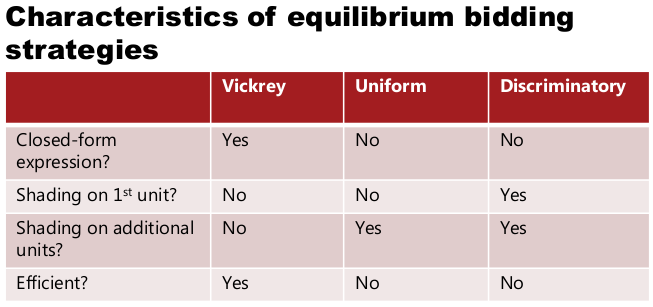
\includegraphics[width=0.6\textwidth]{figures/characteristics.png}
    \caption{\textbf{Characteristics of multiunit formats}}
\end{SCfigure}

\paragraph{Multiunit revenue equivalence}
Let $X^i=(X_1^i, X_2^i, ..., X_K^i)$ be a vector of bidder $i$'s valuations where $X_k^i$ is the marginal valuation of winning the $k$th unit. These are drawn independently from 
\begin{equation}
    \mathcal{X} = \{x \in [0,\omega]^K
    : \forall k, x_k \geq x_{k+1} 
    \}
\end{equation}
potentially with individual densities $f_i:\mathcal{X}\rightarrow [0,1]$. Now fix an auction format with a fixed equilibrium $\bm\beta=(\bm\beta^1, \bm\beta^2, ...,\bm\beta^N)$ assume that all other bidders follow the equilibrium $\bm\beta^j$. Then if bidder $i$ has value vector $\bm{x}^i$ but pretends to have values $\bm{z}^i$ and thus bids $\bm\beta^i(\bm{z}^i)$. We denote by $q_k^i(\bm{z}^i)$ the probability that bidder $i$ wins the $k$th unit, as a function of his pretended value vector. The bidders gain from pretending to have $\bm{z}^i$ can be written 
\begin{equation}
    \sum_{k=1}^K q_k^i(\bm{z}^i)x_k^i = \bm{q}^i(\bm{z}^i) \bm{x}^i
\end{equation}

By two auctions having the same allocation rule we mean exactly that the probabilities $q_k^i(\bm{z}^i)$ are the same in both auctions. Letting $m^i(\bm{z}^i)$ be the expected payment in some auction by bidder $i$ and assume that $m^i(0)=0$. The bidders expected payoff is then 
\begin{equation}
    \Pi(\bm{z}^i,\bm{x}^i) = \bm{q}^i(\bm{z}^i) \cdot \bm{x}^i - m^i(\bm{z}^i)
\end{equation}
and because in equilibrium it is optimal (by definition) to bid $\bm{\beta}^i(\bm{x}^i)$ we have 
\begin{equation}
    \forall \bm{z}^i : \ \bm{q}^i(\bm{x}^i) \cdot \bm{x}^i - m^i(\bm{x}^i) \geq \bm{q}^i(\bm{z}^i) \cdot \bm{x}^i - m^i(\bm{z}^i)
\end{equation}

(See Krishna p.205-206 for continuation, it gets quite complicated)
\\ \\
Following through with the proof it can be shown that the equilibrium payoff functions in two auctions with the same allocation rule are identical up to a constant. The additive constant arises as the payoff for a bidder with value vector $0$, so this falls out when assuming that this is 0. 

\paragraph{Example of applying multiunit revenue equivalence}
Let us consider a case with $K=3$ items for sale, and 2-unit demand from two bidders. The value vector for each bidder is IID $X^i=(X_1^i, X_2^i)$ on $[0,1]^2$, and naturally $X_1^i>X_2^i$. We know that in the Vickrey format it is optimal to submit truthful bids, so 
\begin{equation}
    (b_1^i, b_2^i) = (x_1^i, x_2^i)
\end{equation}
because both bidders have two unit demand, they face competing bids 
\begin{equation}
    c^{-i}  = (x_1^j, x_2^j, 0)
\end{equation}
Both bidders are guaranteed to win one unit, as there are three for sale and each bidder only wants two. One bidder will therefore win two items and pay $x_2^j + 0$, while the other bidder wins one item at a price of $0$. For some given $x_1, x_2$ the expected payment is thus 
\begin{equation}
    m^V(\bm{x}) = P(X_2 < x_2)\cdot E[X_2 | X_2 < x_2] = \int_0^{x_2} y f_2(y) \ dy
\end{equation}
i.e. the other bidders expected bid on the second unit (independence implies we can drop the superscripts), given it is smaller than $x_2$, times the probability this happens. 
\\ \\
Now consider the equivalent uniform auction. We know that the bids here will be $(b_1^i, b_2^i) = (x_1^i, \beta(x_2^i))$. Assuming such a $\beta$ exists and it is increasing we can see that the uniform auction will be efficient. This is in essence because both bidders will certainly win 1 unit, and only win a second if $b_2^i > b_2^j$ implying by monotonicity $x_2^i > x_2^j$. Knowing this the expected payment for bidder $i$ in a uniform auction must be the sum of 1) the expected payment when winning two units, at a price of $x_2^j$ (the highest non-winning bid) and 2) the expected payment when winning one item, which is bidder $i$'s own bid for the second item (the highest non-winning bid) times the probability of this happening, that is 
\begin{equation}
    m^U(\bm{x}) = \int_0^{x_2} 2 \beta(y)f_2(y) \ dy 
    + (1- F_2(x_2)) \beta(x_2)
\end{equation}
Now due to the revenue equivalence theorem (applicable because we have argued that both auctions are efficient) it must be that $\forall z\in[0, \omega]: \ m^V(x_1, z)=m^U(x_1, z)$, i.e.
\begin{equation}
    \int_0^{z} y f_2(y) \ dy = 
    \int_0^{z} 2 \beta(y)f_2(y) \ dy 
    + (1- F_2(z)) \beta(z)   
\end{equation}
Taking the derivative w.r.t $z$ gives 
\begin{equation}
    \begin{split}
    z f_2(z) &= 2 \beta(z) f_2(z) + (1-F_2(z)) \beta'(z) - f_2(z)\beta(z)  \\ 
    &=\beta(z) f_2(z) + (1-F_2(z)) \beta'(z)
    \end{split} 
\end{equation}
Using that $\beta(0)=0$ this can be written as 
\begin{equation}
    \beta'(z) = (z-\beta(z)) \lambda_2(z), \quad \lambda_2(z) \equiv \frac{f_2(z)}{1- F_2(z)}
\end{equation}
Solving this differential equation gives 
\begin{equation}
    \beta(z) = \int_0^z y \lambda_2(y) \ dL(y|z)
\end{equation}
where $L(y|z)=\exp \left(- \int_y^z   \lambda_2(t) \ dt \right)$ which is identical to the integrating factor also used in the single-item auction. Thus we have been able to derive the closed form equilibrium strategy in this very particular case of uniform pricing. 

\paragraph{Discriminatory auction} 
A similar argument for efficiency can be made in the discriminatory price auction, once again on the grounds that in fact only one item is truely "for sale" as bidders only want two each, meaning they get one item free each. Arguing that the demand will be flat in this case and going through the calculations of equating expected payments it can be shown that in this case the bid for both the first and second unit will follow 
\begin{equation}
    \beta(x_2) = \frac{1}{1 + F_2(x_2)} \int_0^{x_2} y f_2(y) \ dy
\end{equation}
which notably does not at all depend on the value of $x_1$.